\section{1174006 - Kadek Diva Krishna Murti}

\subsection{Teori}
\begin{enumerate}
	\item Jelaskan kenapa file teks harus di lakukan tokenizer. dilengkapi dengan ilustrasi atau gambar.\\
	File teks harus dilakukan tokenizer untuk mengkonversi teks menjadi urutan integer indeks kata atau vektor binary, word count atau tf-idf.\\
	Contoh:\\
	texts = ["Diva makan nasi goreng."]\\
	Hasil:\\
	indexs: {'budi': 3, 'nasi': 1, 'makan': 2, 'goreng': 4}

	\item Jelaskan konsep dasar K Fold Cross Validation pada dataset komentar Youtube pada kode listing 7.1. dilengkapi dengan ilustrasi atau gambar.
	\lstinputlisting[firstline=1, lastline=2]{src/1174006/chapter7/teori/listing.py}
	Konsep dasar dalam K Fold Cross Validation, yaitu dataset nantinya dibagi menjadi sejumlah K-buah partisi secara acak. Kemudian dilakukan sejumlah K-kali eksperimen, dimana masing-masing eksperimen menggunakan data partisi ke-K sebagai data testing dan memanfaatkan sisa partisi lainnya sebagai data training.\\
	Pada Listing diatas cara kerjanya yaitu memanggil class StratifiedKFold() lalu tentukan K-nya sebanyak 5 (n\_splits=5). Kemudian data KFold di split sesuai dengan atribut class.
	\item Jelaskan apa maksudnya kode program for train, test in splits.dilengkapi dengan ilustrasi atau gambar.\\
	Kode program for train, test in splits: maksudnya dilakukan perulangan dari data splits dengan variabel train dan test.
	\item Jelaskan apa maksudnya kode program train\_content = d['CONTENT'].iloc[train\_idx] dan test\_content = d['CONTENT'].iloc[test\_idx]. dilengkapi dengan ilustrasi atau gambar.\\
	Kode program train\_content = d['CONTENT'].iloc[train\_idx] maksudnya mengambil data pada atribut content dimana indexnya sesuai dengan train\_idx.\\
	Kode program test\_content = d['CONTENT'].iloc[test\_idx] maksudnya mengambil data pada atribut content dimana indextnya sesuai dengan test\_idx.
	\item Jelaskan apa maksud dari fungsi tokenizer = Tokenizer(num\_words=2000) dan tokenizer.fit\_on\_texts(train\_content), dilengkapi dengan ilustrasi atau gambar.\\
	Fungsi tokenizer = Tokenizer(num\_words=2000) maksudnya memanggil class Tokenizer dengan parameter jumlah kata maksimum untuk disimpan, berdasarkan
	pada frekuensi kata yaitu 2000.\\
	Fungsi tokenizer.fit\_on\_texts(train\_content) maksudnya untuk metraining data text dengan parameter train\_content.
	\item Jelaskan apa maksud dari fungsi d\_train\_inputs = tokenizer.texts\_to\_matrix(train\_content, mode='tfidf') dan d\_test\_inputs = tokenizer.texts\_to\_matrix(test\_content, mode='tfidf'), dilengkapi dengan ilustrasi kode dan atau gambar.\\
	Fungsi d\_train\_inputs = tokenizer.texts\_to\_matrix(train\_content, mode='tfidf') maksudnya mengkoversi list text ke matrix dengan parameter train\_content dan mode tfidf.\\
	Fungsi d\_test\_inputs = tokenizer.texts\_to\_matrix(test\_content, mode='tfidf') maksudnya mengkoversi list text ke matrix dengan parameter test\_content dan mode tfidf.
	\item Jelaskan apa maksud dari fungsi d\_train\_inputs = d\_train\_inputs/np.amax(np.absolute(d\_train\_inputs)) dan d\_test\_inputs = d\_test\_inputs/np.amax(np.absolute(d\_test\_inputs)), dilengkapi dengan ilustrasi atau gambar.\\
	Fungsi d\_train\_inputs = d\_train\_inputs/np.amax(np.absolute(d\_train\_inputs)) maksudnya membagi hasil tfidf dengan nilai maxnya pada d\_train\_inputs.\\
	Fugnsi d\_test\_inputs = d\_test\_inputs/np.amax(np.absolute(d\_test\_inputs)) maksudnya membagi hasil tfidf dengan nilai maxnya pada d\_test\_inputs\\
	\item Jelaskan apa maksud fungsi dari d\_train\_outputs = np\_utils.to\_categorical(d['CLASS'].iloc[train\_idx]) dan d\_test\_outputs = np\_utils.to\_categorical(d['CLASS'].iloc[test\_idx]) dalam kodeprogram, dilengkapi dengan ilustrasi atau gambar.\\
	Fungsi d\_train\_outputs = np\_utils.to\_categorical(d['CLASS'].iloc[train\_idx]) maksudnya mengubah vektor kelas (integer) ke matriks kelas biner sesuai dengan index classnya dari train\_idx.\\
	Fungsi d\_test\_outputs = np\_utils.to\_categorical(d['CLASS'].iloc[test\_idx]) maksudnya  maksudnya mengubah vektor kelas (integer) ke matriks kelas biner sesuai dengan index classnya dari text\_idx.\\
	\item Jelaskan apa maksud dari fungsi di listing 7.2.  Gambarkan ilustrasi Neural Network nya dari model kode tersebut.
	\lstinputlisting[firstline=4, lastline=9]{src/1174006/chapter7/teori/listing.py}
	Maksud fungsi dari listing diatas adalah:
	\begin{itemize}
		\item Mendefinisikan class Sequential()
		\item Memanggil fungsi Dense dengan output array shape 512 dan input array shape 2000
		\item Memanggil fungsi Activation tipe relu
		\item Memanggil fungsi Dropout franction input 0.5
		\item Memanggil fungsi Dense dengan output array shape 2
		\item Memanggil fungsi Activation tipe softmax
	\end{itemize}
	\item Jelaskan apa maksud dari fungsi di listing 7.3 dengan parameter tersebut.
	\lstinputlisting[firstline=11, lastline=12]{src/1174006/chapter7/teori/listing.py}
	Fungsi dari listing diatas maksudnya mengkonfigurasi model untuk dilakukan training.
	\item Jelaskan apa itu Deep Learning.
	Deep learning merupakan metode pembelajaran yang dilakukan oleh mesin dengan cara meniru bagaimana sistem dasar otak manusia bekerja. Deep learning adalah salah satu cabang dari ilmu pembelajaran mesin (Machine Learning) yang terdiri dari algoritma pemodelan abstraksi tingkat tinggi pada data menggunakan sekumpulan fungsi transformasi non-linear yang ditata berlapis-lapis dan mendalam.
	\item Jelaskan apa itu Deep Neural Network, dan apa bedanya dengan Deep Learning.
	Deep Neural Network adalah jaringan saraf tiruan yang memiliki beberapa lapisan antara lapisan input dan lapisan output. Perbedaan dari Deep Neural Network dan Deep Learning adalah Deep Neural Network merupakan metode yang digunakan sebagai pembelajaran oleh Deep Learning.
	\item Jelaskan dengan ilustrasi gambar buatan sendiri (langkah per langkah) bagaimana perhitungan algoritma konvolusi dengan ukuran stride (NPM mod3+1) x (NPM mod3+1) yang terdapat max pooling.
\end{enumerate}
\subsection{Praktek}
\begin{enumerate}
	\item Jelaskan kode program pada blok \ In[1]. Jelaskan arti dari setiap baris kode yang dibuat (harus beda dengan teman sekelas) dan hasil luarannya dari komputer sendiri.
	\hfill\break

	\lstinputlisting[firstline=1, lastline=15]{src/1174006/chapter7/praktek/praktek.py}
	% \begin{figure}[H]
	% 	\includegraphics[width=8cm]{figures/1174006/chapter7/praktek/xxx.png}
	% 	\centering
	% \end{figure}

	\item Jelaskan kode program pada blok  In[2]. Jelaskan arti dari setiap baris kode yang dibuat (harus beda dengan teman sekelas) dan hasil luarannya dari komputer sendiri.
	\hfill\break

	\lstinputlisting[firstline=17, lastline=33]{src/1174006/chapter7/praktek/praktek.py}
	% \begin{figure}[H]
	% 	\includegraphics[width=8cm]{figures/1174006/chapter7/praktek/xxx.png}
	% 	\centering
	% \end{figure}

	\item Jelaskan kode program pada blok  In[3]. Jelaskan arti dari setiap baris kode yang dibuat (harus beda dengan teman sekelas) dan hasil luarannya dari komputer sendiri.
	\hfill\break

	\lstinputlisting[firstline=35, lastline=40]{src/1174006/chapter7/praktek/praktek.py}
	% \begin{figure}[H]
	% 	\includegraphics[width=8cm]{figures/1174006/chapter7/praktek/xxx.png}
	% 	\centering
	% \end{figure}

	\item Jelaskan kode program pada blok  In[4]. Jelaskan arti dari setiap baris kode yang dibuat (harus beda dengan teman sekelas) dan hasil luarannya dari komputer sendiri.
	\hfill\break

	\lstinputlisting[firstline=42, lastline=49]{src/1174006/chapter7/praktek/praktek.py}
	% \begin{figure}[H]
	% 	\includegraphics[width=8cm]{figures/1174006/chapter7/praktek/xxx.png}
	% 	\centering
	% \end{figure}

	\item Jelaskan kode program pada blok  In[5]. Jelaskan arti dari setiap baris kode yang dibuat (harus beda dengan teman sekelas) dan hasil luarannya dari komputer sendiri.
	\hfill\break

	\lstinputlisting[firstline=51, lastline=51]{src/1174006/chapter7/praktek/praktek.py}
	% \begin{figure}[H]
	% 	\includegraphics[width=8cm]{figures/1174006/chapter7/praktek/xxx.png}
	% 	\centering
	% \end{figure}

	\item Jelaskan kode program pada blok  In[6]. Jelaskan arti dari setiap baris kode yang dibuat (harus beda dengan teman sekelas) dan hasil luarannya dari komputer sendiri.
	\hfill\break

	\lstinputlisting[firstline=53, lastline=57]{src/1174006/chapter7/praktek/praktek.py}
	% \begin{figure}[H]
	% 	\includegraphics[width=8cm]{figures/1174006/chapter7/praktek/xxx.png}
	% 	\centering
	% \end{figure}

	\item Jelaskan kode program pada blok  In[7]. Jelaskan arti dari setiap baris kode yang dibuat (harus beda dengan teman sekelas) dan hasil luarannya dari komputer sendiri.
	\hfill\break

	\lstinputlisting[firstline=59, lastline=62]{src/1174006/chapter7/praktek/praktek.py}
	% \begin{figure}[H]
	% 	\includegraphics[width=8cm]{figures/1174006/chapter7/praktek/xxx.png}
	% 	\centering
	% \end{figure}

	\item Jelaskan kode program pada blok  In[8]. Jelaskan arti dari setiap baris kode yang dibuat (harus beda dengan teman sekelas) dan hasil luarannya dari komputer sendiri.
	\hfill\break

	\lstinputlisting[firstline=64, lastline=73]{src/1174006/chapter7/praktek/praktek.py}
	\begin{figure}[H]
		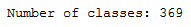
\includegraphics[width=8cm]{figures/1174006/chapter7/praktek/8.png}
		\centering
	\end{figure}

	\item Jelaskan kode program pada blok  In[9]. Jelaskan arti dari setiap baris kode yang dibuat (harus beda dengan teman sekelas) dan hasil luarannya dari komputer sendiri.
	\hfill\break

	\lstinputlisting[firstline=75, lastline=75]{src/1174006/chapter7/praktek/praktek.py}
	% \begin{figure}[H]
	% 	\includegraphics[width=8cm]{figures/1174006/chapter7/praktek/xxx.png}
	% 	\centering
	% \end{figure}

	\item Jelaskan kode program pada blok  In[10]. Jelaskan arti dari setiap baris kode yang dibuat (harus beda dengan teman sekelas) dan hasil luarannya dari komputer sendiri.
	\hfill\break

	\lstinputlisting[firstline=77, lastline=92]{src/1174006/chapter7/praktek/praktek.py}
	\begin{figure}[H]
		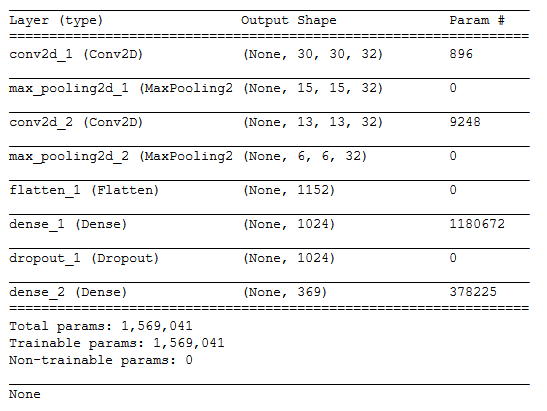
\includegraphics[width=8cm]{figures/1174006/chapter7/praktek/10.png}
		\centering
	\end{figure}

	\item Jelaskan kode program pada blok  In[11]. Jelaskan arti dari setiap baris kode yang dibuat (harus beda dengan teman sekelas) dan hasil luarannya dari komputer sendiri.
	\hfill\break

	\lstinputlisting[firstline=94, lastline=96]{src/1174006/chapter7/praktek/praktek.py}
	% \begin{figure}[H]
	% 	\includegraphics[width=8cm]{figures/1174006/chapter7/praktek/xxx.png}
	% 	\centering
	% \end{figure}

	\item Jelaskan kode program pada blok  In[12]. Jelaskan arti dari setiap baris kode yang dibuat (harus beda dengan teman sekelas) dan hasil luarannya dari komputer sendiri.
	\hfill\break

	\lstinputlisting[firstline=98, lastline=108]{src/1174006/chapter7/praktek/praktek.py}
	\begin{figure}[H]
		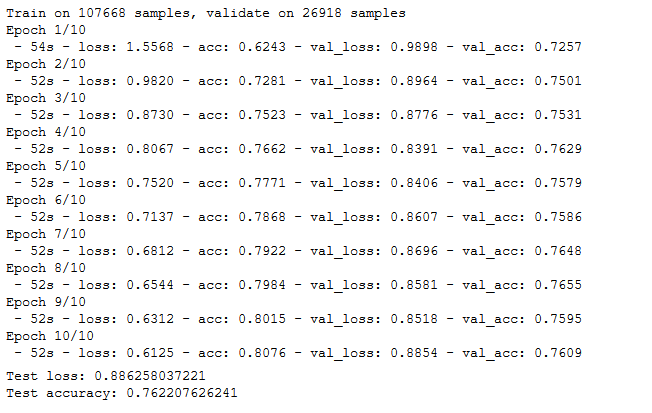
\includegraphics[width=8cm]{figures/1174006/chapter7/praktek/12.png}
		\centering
	\end{figure}

	\item Jelaskan kode program pada blok  In[13]. Jelaskan arti dari setiap baris kode yang dibuat (harus beda dengan teman sekelas) dan hasil luarannya dari komputer sendiri.
	\hfill\break

	\lstinputlisting[firstline=110, lastline=147]{src/1174006/chapter7/praktek/praktek.py}
	\begin{figure}[H]
		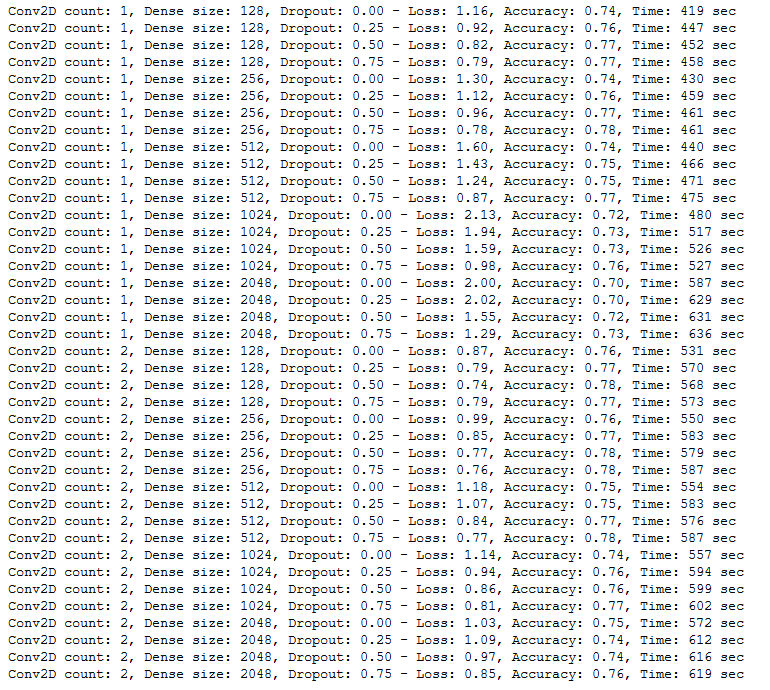
\includegraphics[width=8cm]{figures/1174006/chapter7/praktek/13.png}
		\centering
	\end{figure}

	\item Jelaskan kode program pada blok  In[14]. Jelaskan arti dari setiap baris kode yang dibuat (harus beda dengan teman sekelas) dan hasil luarannya dari komputer sendiri.
	\hfill\break

	\lstinputlisting[firstline=150, lastline=163]{src/1174006/chapter7/praktek/praktek.py}
	\begin{figure}[H]
		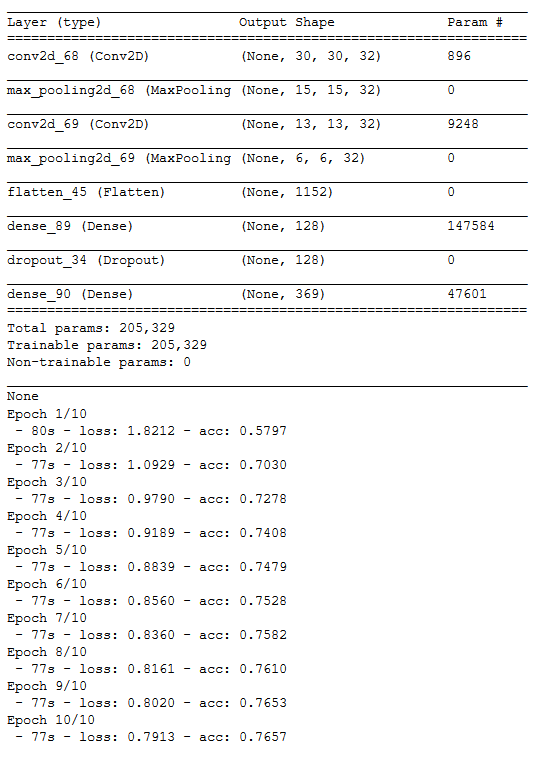
\includegraphics[width=8cm]{figures/1174006/chapter7/praktek/14.png}
		\centering
	\end{figure}

	\item Jelaskan kode program pada blok  In[15]. Jelaskan arti dari setiap baris kode yang dibuat (harus beda dengan teman sekelas) dan hasil luarannya dari komputer sendiri.
	\hfill\break

	\lstinputlisting[firstline=164, lastline=167]{src/1174006/chapter7/praktek/praktek.py}
	% \begin{figure}[H]
	% 	\includegraphics[width=8cm]{figures/1174006/chapter7/praktek/xxx.png}
	% 	\centering
	% \end{figure}

	\item Jelaskan kode program pada blok  In[16]. Jelaskan arti dari setiap baris kode yang dibuat (harus beda dengan teman sekelas) dan hasil luarannya dari komputer sendiri.
	\hfill\break

	\lstinputlisting[firstline=169, lastline=170]{src/1174006/chapter7/praktek/praktek.py}
	% \begin{figure}[H]
	% 	\includegraphics[width=8cm]{figures/1174006/chapter7/praktek/xxx.png}
	% 	\centering
	% \end{figure}

	\item Jelaskan kode program pada blok  In[17]. Jelaskan arti dari setiap baris kode yang dibuat (harus beda dengan teman sekelas) dan hasil luarannya dari komputer sendiri.
	\hfill\break

	\lstinputlisting[firstline=172, lastline=173]{src/1174006/chapter7/praktek/praktek.py}
	% \begin{figure}[H]
	% 	\includegraphics[width=8cm]{figures/1174006/chapter7/praktek/xxx.png}
	% 	\centering
	% \end{figure}

	\item Jelaskan kode program pada blok  In[18]. Jelaskan arti dari setiap baris kode yang dibuat (harus beda dengan teman sekelas) dan hasil luarannya dari komputer sendiri.
	\hfill\break

	\lstinputlisting[firstline=176, lastline=180]{src/1174006/chapter7/praktek/praktek.py}
	\begin{figure}[H]
		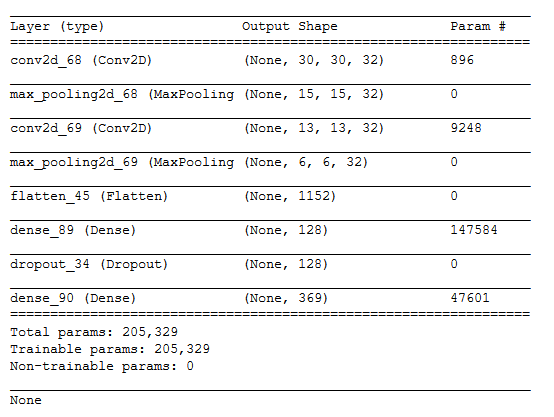
\includegraphics[width=8cm]{figures/1174006/chapter7/praktek/18.png}
		\centering
	\end{figure}

	\item Jelaskan kode program pada blok  In[19]. Jelaskan arti dari setiap baris kode yang dibuat (harus beda dengan teman sekelas) dan hasil luarannya dari komputer sendiri.
	\hfill\break

	\lstinputlisting[firstline=182, lastline=198]{src/1174006/chapter7/praktek/praktek.py}
	% \begin{figure}[H]
	% 	\includegraphics[width=8cm]{figures/1174006/chapter7/praktek/xxx.png}
	% 	\centering
	% \end{figure}

	\item Jelaskan kode program pada blok  In[20]. Jelaskan arti dari setiap baris kode yang dibuat (harus beda dengan teman sekelas) dan hasil luarannya dari komputer sendiri.
	\hfill\break

	\lstinputlisting[firstline=201, lastline=206]{src/1174006/chapter7/praktek/praktek.py}
	\begin{figure}[H]
		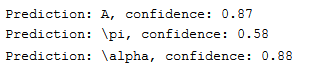
\includegraphics[width=8cm]{figures/1174006/chapter7/praktek/20.png}
		\centering
	\end{figure}

\end{enumerate}

\subsection{Penanganan Error}

\subsection{Bukti Tidak Plagiat}
\begin{figure}[H]
	
\includegraphics[width=4cm]{kreatiflogo.png}
	\centering
	\caption{Kecerdasan Buatan.}
\end{figure}